\cleardoublepage
\clearpage{}

%[Lo que va en el índice]{Lo que va en el documento}
\chapter[Metodología de trabajo]{Metodología de trabajo}
\section{Metodología de trabajo seguida en el documento}
Desde el comienzo del trabajo se ha seguido una  metodología ágil. Cada semana o cada dos semanas se celebraba una reunión con el tutor, vía Google Meet, por norma general. En dichas reuniones se exponía el trabajo realizado tras la reunión anterior y se resolvían las dudas surgidas. Además, se proponían una serie de objetivos que, deseablemente había que trabajar de cara a la siguiente reunión. Gracias a seguir esta forma de organización, se logró avanzar en el proyecto de la forma deseada. \\

Con el fin de tener un registro de como iba avanzando la memoria, se creó un repositorio en  \href{http://www.github.com}{\textit{Github}} (\url{github.com/aguillenATC/TFG-Mena-Sistemas-de-Archivos}). Dicho repositorio esta enlazado con el proyecto alojado en \href{http://www.overleaf.com}{\textit{Overleaf}} y al final de cada sesión de trabajo se actualizaban los cambios. No obstante, las primeras versiones del documento no se encuentran registradas en el repositorio debido a la implantación a posteriori de este sistema.\\

En referencia a la búsqueda de información, el objetivo era primar la información de calidad, para ello siempre se ha tratado de acudir a documentaciones oficiales (si estaban disponibles) o directamente consultar bibliografía. En caso de que esto no fuera posible, el siguiente paso era la búsqueda información de empresas relacionadas con la cuestión a tratar (por ejemplo: Ext4 la documentación oficial disponible es muy escueta, mientras que la información disponible en la página de Fedora es bastante completa). Por último, la revisión en \textit{papers} que en algunos casos cuentan con información muy buena y completa.

\section{Metodología de los experimentos}
Tal como se mencionó con anterioridad, el objetivo de este trabajo consiste en comparar el rendimiento de Btrfs, Ext4 y XFS en un único disco. Para realizar la comparativa de rendimiento, se debe plantear el uso de distintas herramientas de \textit{benchmarking} que sean capaces de evaluar el comportamiento bajo una determinada carga. En este contexto de estudio existen dos tipos de \textit{benchmarks}. \\

Por un lado tenemos \textit{benchmarks} reales (medir el rendimiento de una tarjeta gráfica utilizando un videojuego). El uso de este tipo de \textit{benchmarks} tiene aspectos positivos, pero resulta difícil encontrar aplicaciones suficientemente representativas que engloben el funcionamiento de un sistema en todas la situaciones.\\

Por otro lado tenemos los \textit{benchmarks} sintéticos. Son programas artificiales que no realizan ningún trabajo real y útil. Las operaciones realizadas por estos \textit{benchmarks} se eligen cuidadosamente para que coincidan con las operaciones que realizarían otro tipo de programas. El objetivo es que las operaciones que realiza el \textit{benchmark} sean lo mas similares posible para así poder exportar los resultados al mundo real \cite{lilja_2000}.\\

La combinación de ambos tipos de \textit{benchmarks} para la medición de rendimiento de E/S del sistema de archivos producirá un resultado más representativo en lugar de depender únicamente de uno de los dos tipos de herramientas. Este proyecto hace uso tanto de \textit{benchmarks} sintéticos elaborados con \textit{Filebench} e \textit{Iozone}, como de aplicaciones reales para las medidas.

\subsection{Entorno de pruebas y repetición de experimentos}\label{numejecs}
El estado del sistema a la hora de ejecutar las pruebas puede influir en los resultados. Poniendo un ejemplo, tal y como señala Avishay Traeger \cite{traeger} el estado de la caché a la hora de ejecutar un test resulta determinante. No está del todo claro la metodología a seguir en estos casos, por un lado en un entorno real la caché no estaría completamente fría\footnote{Caché fría: Cuando la caché está vacía o contiene datos irrelevantes, esta situación conlleva hacer lecturas desde memoria principal.}. Por otro lado, un \textit{benchmark} que accede a demasiados datos que se encuentran almacenados en caché también es poco realista. Si deseamos resultados de caché fría, habrá que desmontar el sistema de archivos tras cada ejecución para asegurar que la caché queda limpia tanto la del disco como la de la CPU \cite{traeger}.\\

Haciendo referencia de nuevo a Avishay Traeger, se establecen cuatro pautas importantes \cite{traeger} a la hora de ejecutar un \textit{benchmark}: 

\begin{enumerate}
    \item Asegurar que cada vez que se ejecuta un \textit{benchmark} sea bajo idéntica configuración.
    \item Cada prueba debe realizarse varias veces para garantizar la precisión. Los niveles de confianza deben utilizarse para determinar el número adecuado de ejecuciones.
    \item Las pruebas se deben realizar durante un periodo de tiempo lo suficientemente largo.
    \item El proceso de \textit{benchmarking} debe automatizarse utilizando scripts u otras herramientas de automatización.
\end{enumerate}

Poniendo el foco en la segunda pauta, es importante que el número de mediciones sea el mínimo sin que esto afecte a la calidad de los resultados. Basándonos en la fórmula de los intervalos de confianza se determinaran cuantas medidas son necesarias para producir un intervalo de una anchura específica \cite{lilja_2000}. \\

Suponiendo que se quiere definir un intervalo de confianza para $\Bar{x}$, hay una probabilidad de $1-\alpha$ de que el valor actual de $x$ esté contenido en el intervalo  $$
\left(c_{1}, c_{2}\right)=((1-e) \bar{x},(1+e) \bar{x})
$$ 
Entonces se tiene que 
$$
c_{1}=(1-e) \bar{x}=\bar{x}-z_{1-\alpha / 2} \frac{s}{\sqrt{n}}
$$
$$
c_{2}=(1+e) \bar{x}=\bar{x}+z_{1-\alpha / 2} \frac{s}{\sqrt{n}}
$$
Como ambos intervalos son simétricos se puede utilizar cualquiera de las dos ecuaciones para determinar que:
$$
z_{1-\alpha / 2} \frac{s}{\sqrt{n}}=\bar{x} e
$$
Despejando $n$ se obtendría
\begin{equation}
\label{eqn:n-ejecuciones}
n=\left(\frac{z_{1-\alpha / 2} s}{e \bar{x}}\right)^{2}
\end{equation}
 

Para determinar el número de mediciones se requiere una estimación de la desviación estándar ($s$). Sin embargo,  dicha desviación no puede ser calculada hasta que se realicen algunas mediciones. Por tanto, el procedimiento consiste en realizar un número relativamente pequeño de mediciones para obtener una estimación de la desviación y la media\cite{lilja_2000}. 


\section{Test Anova}\label{anova_section}
Una vez se han ejecutado las pruebas el número de veces necesarias, se podrán adquirir suficientes simulaciones para llegar a conclusiones estadísticamente significativas. Dichos resultados podrían ser debidos al cambio de factor en la alternativa o por cuestiones de ruido en la medición. Debido a ello se hará uso del test anova (\textit{\textbf{An}alisys \textbf{o}f \textbf{Va}riance})\\

El análisis de varianza es una técnica para dividir la variación de unas mediciones y convertirla en mediciones significativas. Este tipo de análisis asume que los errores en las mediciones de las distintas alternativas son independientes y siguen una distribución gaussiana (distribución normal). Se supone que la varianza del error es la misma para todas las alternativas. El test Anova divide la variación en dos: por un lado la variación causada por los errores en las mediciones y por otro lado la variación entre sistemas. El objetivo es determinar si la variación entre sistemas se debe a la diferencia real entre dichos sistemas o simplemente es debido a error en la medición. \cite{lilja_2000} \\

¿Las diferencias entre las medidas observadas para las alternativas se deben a diferencias reales entre las alternativas, o se deben simplemente a errores de medición? 
Para resolver esta cuestión, se requieren $n$ mediciones en cada una de las $k$ alternativas. Según Lilja \cite{lilja_2000} es conveniente organizar las mediciones en una tabla cómo la siguiente. 
 
\begin{figure}[H]
    \centering
    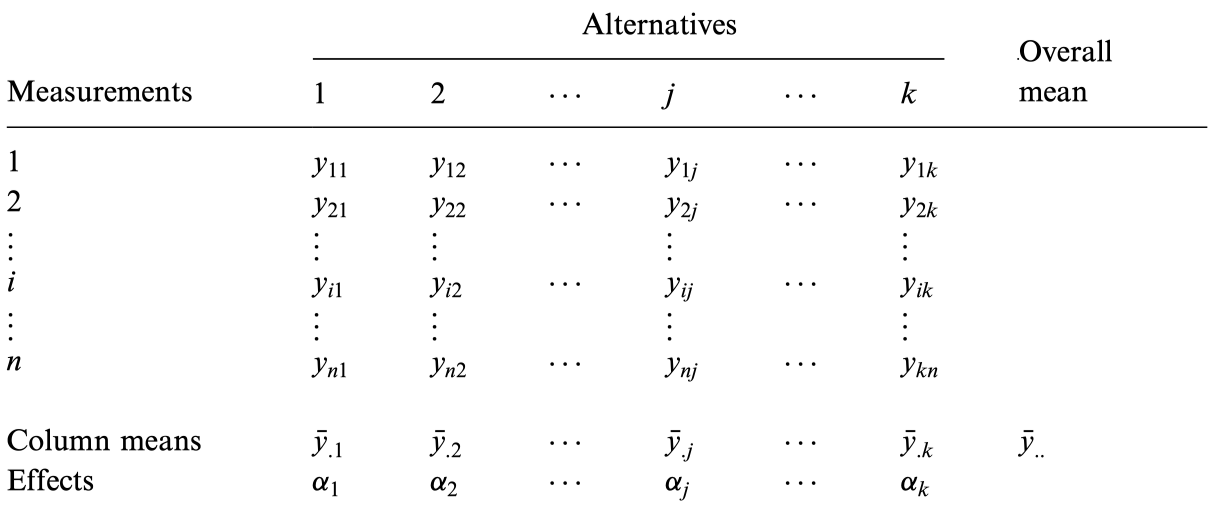
\includegraphics[scale=0.6]{doc/assets/images/Capitulo3/lilja_recommend.png}
    \caption{Ordenación de las mediciones para facilitar los cálculos del test Anova \cite{lilja_2000}}
    \label{fig:Anova_liljal}
\end{figure}

Dónde $y_{ij}s$ es la i-ésima medida de la j-ésima alternativa. La fila de la media de las columnas se denomina $\Bar{y}_{.j}$ y se calcula como $
\bar{y}_{. j}=\frac{\sum_{i=1}^{n} y_{i j}}{n}
$. La media total $\Bar{y}_{..}$ es la media de todas las medidas realizadas en todas las alternativas cuya fórmula sería $$
\bar{y}_{. .}=\frac{\sum_{j=1}^{n} \sum_{i=1}^{n} y_{i j}}{k n}
$$.

Es útil descomponer cada medida $y_{ij}$ como la suma de todas las medias de la alternativa $j$, $\bar{y}_{.j}$ y un valor $e_{ij}$ que representa la desviación de la medición respecto a la media. Por lo que partiendo de este enunciado la ecuación resultante es: $$y_{ij}=\bar{y}_{.j} + e_{ij}$$.

Se puede extender este razonamiento para representar la fila de medias $\bar{y}_{ij}$ como la suma de la media total $\bar{y}_{..}$ y la desviación de la fila de las medias $\alpha_j$. Como resultado se obtiene: $$
y_{i j}=\bar{y}_{. .}+\alpha_{j}+e_{i j}
$$

Expresar las medidas de esta forma permite dividir la variación de todas las medidas en dos componentes separados. Por un lado la variación provocada por los efectos de las alternativas y por otro lado la variación debida a los errores. Respecto a la variación debida a los efectos de las alternativas, la cual no se debe confundir con la varianza, comúnmente denominada \textit{SSA} y  calculada de la siguiente forma:  $$S S A=n \sum_{j=1}^{k}\left(\bar{y}_{. j}-\bar{y}_{. .}\right)^{2}$$. 

De forma similar la variación debida a errores se denota como \textit{SSE}. Calculada como la sumatoria del cuadrado de las diferencias entre las medidas individuales y su correspondiente media total. De este modo se tiene que:  $$S S E=\sum_{j=1}^{k} \sum_{i=1}^{n}\left(y_{i j}-\bar{y}_{. j}\right)^{2}$$ 

Finalmente, la varianza residual se calcula como:
$$
S S T=\sum_{j=1}^{k} \sum_{i=1}^{n}\left(y_{i j}-\bar{y}_{..}\right)^{2}
$$

De todo esto se puede deducir que $$S S T= S S A + S S E$$

El objetivo es contrastar la hipótesis de que el factor no influye sobre los resultados. Si esto es así, el resultado de calcular $F_{exp}$ debería ser una muestra de una distribucion F de Snedecor.

$$
F_{e x p} = \frac{\operatorname{SSA} /\left(k-1\right)}{\operatorname{SSE} /\left (k(n-1)\right) } \sim F_{k-1,k(n-1)}
$$
\\
La prueba estadística que ha demostrado ser adecuada para este tipo de comparativas es el test-F. Este test, que se basa en la distribución F de Snedecor, se utiliza para comprobar si dos varianzas son significativamente diferentes. Dado que el estadístico F se calcula como el cociente de dos varianzas, los valores cercanos a 1 indicarán que probablemente no existe ninguna diferencia significativa.\\

Las estimaciones de las varianzas de $SSA$ y $SSE$ se hallan calculando sus correspondientes valores de \textit{mean-square}. El \textit{mean-square} es simplemente la variación total del componente dividida por el número de grados de libertad de ese componente. Dado que se comparan $k$ alternativas, hay $k-1$ grados de libertad en $SSA$. Por lo que, la estimación de la varianza es: $$
s_{\mathrm{a}}^{2}=\frac{S S A}{k-1}
$$

De forma similar ocurre con $SSE$, como cada una de las alternativas tiene n-mediciones, cada alternativa tiene $n-1$ grados de libertad. Por lo tanto, el número total de grados de libertad para $SSE$ es $kn-1$, ya que hay k alternativas. La estimación de la varianza del error es entonces: 
$$
s_{\mathrm{a}}^{2}=\frac{S S E}{k(n-1)}
$$

Finalmente el estadístico $F$ para este test es calculado de la siguiente manera: $$
F=\frac{s_{\mathrm{a}}^{2}}{s_{\mathrm{e}}^{2}}
$$

Dado que el estadístico $F$ es calculado como el cociente de dos varianza necesitará de dos valores para los grados de libertad. Si el valor de F calculado es mayor que el valor $F_{[1-\alpha ;(k-1), k(n-1)]}$ obtenido de la tabla, la variación causada entre las alternativas es mayor que la causada por los errores en un nivel de confianza de $1-\alpha$.



\section{Máquina de pruebas}
Los experimentos fueron ejecutados en una máquina convencional con un procesador AMD con una frecuencia de reloj de 3.5 GHz. Ubuntu 16.04.7 es la versión del sistema operativo en la que se ejecutan las pruebas. El sistema tiene 2 discos, en un disco SSD se encuentra el sistema operativo y las herramientas de \textit{benchmarking} y en el disco duro mecánico se utiliza exclusivamente para el montaje de los sistemas de archivos. La tabla siguiente muestra todos los detalles sobre el hardware y software utilizado.
\begin{table}[h]
    \centering
    \begin{tabular}{|l|l|}
    \hline
        Componente & Modelo \\ \hline\hline
        CPU & AMD Ryzen 3 1300X @ 3.5 GHz Quad-Core \\ \hline
        Memoria & Crucial CT8G4DFS824A. 8 GB DDR4 2400 MHz CL17 \\ \hline
        Placa Base & ASUS EX-A320M \\ \hline
        SSD del Sistema & Kingston A400 SSD SATA3 \textcolor{blue}{¿Prestaciones de velocidad?} \\ \hline
        HDD de Pruebas & Seagate Barracuda ST500DM002-1BD14 500GB \textcolor{blue}{¿Prestaciones de velocidad?}\\ \hline
    \end{tabular}
    \caption{Especificaciones Hardware \textcolor{blue}{QUIZÁS AÑADIR UNA COLUMNA ESPECIFICACIONES CON LAS MÁS RESEÑABLES DE CADA COMPONENTE}}
\label{table:1}
\end{table}

\begin{table}[H]
    \centering
    \begin{tabular}{|l|l|}
    \hline
        Software & Versión \\ \hline\hline
        Ubuntu 18.04.5 LTS & Kernel GNU/Linux 5.4.0-42-generic x86\_64 \\ \hline
        Filebench & 1.5-alpha3 \\ \hline
        KownSeq & 1.6.0 \\ \hline
        iozone & 3.429 \\ \hline
        R & v4.1.0 (2021-05-18) \\ \hline
    \end{tabular}
    \caption{Especificaciones Software}
\label{table:2}
\end{table}

\subsection{Montaje de los sistemas de archivos}
El sistema de archivos que monta el disco que alberga el sistema operativo es Ext4, no existe ningún motivo que justifique el uso de este sistema concreto \textcolor{blue}{NO ENTIENDO ESTA FRASE, ¿PORQUE JUSTIFICAS QUE NO HAY MOTIVO QUE JUSTIFIQUE EL USO DE EXT4? CON DECIR QUE SE HA USADO ESE POR SER EL MAS ESTANDAR EN ESTE TIPO DE DISTROS Y QUE LAS PRUEBAN VAN EN EL OTRO COMO DICES DESPUES BASTARIA}, ya que las pruebas se ejecutan en otro dispositivo distinto. \\

El disco en el que se ejecutan las pruebas dispone de una sola partición que ocupa el total de la capacidad del disco. Los sistemas de archivos (Ext4, BTRFS y XFS) se crean con la herramienta \textit{mkfs}. Tras la lectura de las opciones disponibles en el manual de la herramienta \cite{tso} \textcolor{purple}{\sout{decidimos}} \textcolor{blue}{se decide} montar los sistemas de archivos con la configuración por defecto, ya que la \textcolor{blue}{propia} herramienta, basándose en los recursos de la máquina, los ajusta.\\

Las orden utilizada para montar un sistema ext4 en la máquina es:

\begin{lstlisting}[language=bash]
 sudo mkfs.ext4 -F -O ^64bit -L '' '/dev/sda1'
\end{lstlisting}

Para la creación de los sistemas XFS y BTRFS  se necesitan instalar las herramientas \textcolor{magenta}{necesarias, como pueden ser  librerías de compresión de datos o librerías de C \cite{lib-ubuntu-btrfs}}. \textcolor{blue}{¿QUE HERRAMIENTAS? MENCIONA ALGO QUE QUEDA MUY VAGO}, estas no vienen en la instalación por defecto en esta versión del sistema operativo. El primer paso antes de instalar las herramientas es actualizar los repositorios.
\begin{lstlisting}[language=bash]
sudo apt-get update
\end{lstlisting}

Tras esto, únicamente tenemos que ejecutar en la terminal la siguiente orden para instalar las herramientas para la creación de un sistema BTRFS:
\begin{lstlisting}[language=bash]
sudo apt-get install btrfs-tools
\end{lstlisting}
Y ya se podría crear el sistema de archivos BTRFS.
\begin{lstlisting}[language=bash]
sudo mkfs.btrfs -f  -L '' '/dev/sda1'
\end{lstlisting}
Tras la ejecución de la orden, se muestra un resumen del sistema de archivos creado.
\begin{lstlisting}[language=bash]
btrfs-progs v4.15.1
See http://btrfs.wiki.kernel.org for more information.

Label:
UUID:               bab5f23b-0092-40bc-8d80-baeeef6f6a5b
Node size:          16384
Sector size:        4096
Filesystem size:    465.76GiB
Block group profiles:
  Data:             single            8.00MiB
  Metadata:         DUP               1.00GiB
  System:           DUP               8.00MiB
SSD detected:       no
Incompat features:  extref, skinny-metadata
Number of devices:  1
Devices:
   ID        SIZE  PATH
    1   465.76GiB  /dev/sda1

\end{lstlisting}

\textcolor{blue}{ESTAS DOS FRASES ESTÁN RARAS, UNIFICALAS Y DEJALO MAS ELEGANTE :)} \textcolor{magenta}{Tal y como ocurre al crear un S.A BTRFS, se necesita disponer de las bibliotecas y herramientas incluidas en el paquete \textit{xfsprogs} \cite{xfsprogs}. Para obtener dicho paquete es necesario ejecutar la siguiente orden en un terminal.}
\begin{lstlisting}[language=bash]
sudo apt-get install xfsprogs
\end{lstlisting}
Y ya podremos crear el sistema de archivos BTRFS.
\begin{lstlisting}[language=bash]
sudo mkfs.xfs -f  -L '' '/dev/sda1'
\end{lstlisting}

Crear particiones, sistemas de ficheros y montarlos de manera manual para poder lanzar las pruebas, es un proceso muy tedioso. Por ello se ha desarrollado un script en bash para la automatización de dicha tarea. El código del script está disponible en la sección \ref{montaje.sh}.

\section{Herramientas de \textit{benchmarking} y metodología}
\subsection{Iozone}\label{metodologia_iozone}
Iozone en general es utilizado para medir el rendimiento del sistema de archivos, utilizando distintos tipos de pruebas. Se utilizará esta herramienta para medir el rendimiento en operaciones de lectura, escritura, re-lectura, re-escritura, lectura aleatoria y escritura aleatoria. Estas opciones se han seleccionado debido a que son operaciones que ejecutan las aplicaciones bajo cualquier tipo de carga.

Los ajustes que se van a utilizar para la configuración de las pruebas son exactamente iguales para ext4, btrfs y xfs. La salida de \textit{iozone} se compone de una tabla donde cada fila \textcolor{blue}{contiene} el tamaño de archivo con el que se ejecuta el test y las columna es el tamaño de bloque. \\

Se realizarán varías ejecuciones con el fin de obtener un promedio y desviación estándar. Una vez tengamos esos datos, se podrá aplicar la fórmula \ref{eqn:n-ejecuciones} para obtener el número de pruebas necesarias.\\

Tras ello se realizarán tests Anova para comprobar si el tamaño de bloque o el tamaño de archivo afecta a la productividad. También se realizarán test correspondientes encargados de determinar si el uso de un S.A (sistema de archivos) \textcolor{blue}{S.A. YA ESTA DEFINIDO ANTERIORMENTE, UNIFICALO CON EL RESTO DEL DOCUMENTO} otro influye en la productividad.



\subsection{Filebench}
\textcolor{purple}{\sout{Utilizaremos}} \textcolor{blue}{Filebench fue seleccionada} \textcolor{purple}{\sout{esta herramienta}} principalmente por disponer de un lenguaje para modelar carga. \textcolor{purple}{\sout{Es decir, utilizaremos \textit{Filebench} \textit{WML} para crear benchmarks.}} El objetivo es crear un benchmark, que simule un uso del disco por parte de una aplicación genérica.\\

Se procederá de la manera similar que con la aplicación \textit{iozone}.

\textcolor{blue}{NO VENDRÍA MAL UN DIAGRAMA DE COMO VAS A ORGANIZAR ESTE BENCHMARK, ADEMÁS DE EXPLICARLO MÁS EN DETALLE. LA PARTE DE KNOWSEQ ESTÁ MUCHO MAS COMPLETA QUE ESTA MINI-SECCIÓN.}

\subsection{KnowSeq}\label{metodologia_knowseq}
KnowSeq es una herramienta que permite procesar y extraer biomarcadores relevantes \textcolor{blue}{partiendo de datos de expresión de gen}, así como evaluarlos mediante enfoques de Machine Learning. El objetivo de KnowSeq es la extracción de conocimiento biológico a partir de biomarcadores \textcolor{blue}{génicos}. \\

El \textcolor{purple}{\sout{primer}} \textcolor{blue}{workflow} del programa se encarga del tratamiento de los datos en crudo. Este proceso consiste en extraer un conjunto de archivos provenientes de los datos en bruto alojados en internet. \textcolor{purple}{\sout{Partimos}} \textcolor{blue}{Primero se parte} de unos archivos SRA y el objetivo es procesarlos para obtener unos ficheros llamados \textit{count files}. La transformación de un archivo SRA a \textit{count file} no es directa, si no que existen pasos intermedios que generan por tanto archivos intermedios. Estos ficheros se denominan \textit{FASTQ, BAM y SAM Files} y son archivos muy pesados (del orden de 10-15 GB). KnowSeq conforme va generando los FASTQ, BAM, SAM Files los va organizando en carpetas, es decir mueve archivos pesados, por lo que durante el proceso se hacen operaciones muy pesadas en el sistema de archivos. Para esta prueba \textcolor{purple}{\sout{obviaremos}} \textcolor{blue}{se obvia} la parte final del proceso que consiste generar los \textit{count files} a partir de los \textit{SAM files}. Este proceso es muy pesado para el procesador, pero apenas hace uso del disco, y debido a ello se decide descartar su uso.\\

\textcolor{blue}{DEBERÍAS HACER UN DIAGRAMA COMO EL QUE TE MOSTRÉ DE COMO PASAR DE UN ARCHIVO A OTRO Y EN QUÉ ORDEN PARA ACLARARLO DE FORMA GRÁFICA.}

Para esta prueba \textcolor{purple}{\sout{utilizaremos}} \textcolor{blue}{se hacen uso de} series relativas al Covid-19. KnowSeq en su repositorio tiene datos de 90 pacientes, pero desafortunadamente se utilizarán sólo datos de 5 de ellos, ya que al ser archivos tan pesados \textcolor{purple}{\sout{necesitaríamos}} \textcolor{blue}{se requeriría de} una cantidad de espacio que no \textcolor{purple}{\sout{disponemos}} \textcolor{blue}{se tiene} y el tiempo de procesamiento es demasiado elevado. \textcolor{blue}{ESTO SE ENTIENDE MAL, DALE UNA VUELTECILLA A LA FRASE}La variación en los genes es uno de los factores que modificaría el tiempo de ejecución, pero que dicha diferencia en los archivos elegidos es pequeña y, por tanto, la diferencia en el tiempo de ejecución también debería serla. Además al procesar los datos de cada paciente de uno en uno y siendo operaciones completamente aisladas entre pacientes, ello supone que el tiempo y las operaciones por cada uno de estos, es prácticamente el mismo. Por lo tanto, se puede asumir que el tiempo y espacio total utilizado se incrementa aproximadamente de forma lineal cada vez que se añade un paciente. Para confirmar esta hipótesis se lanzaron varias ejecuciones (3 por configuración) del programa con distinto número de pacientes, con el fin de determinar si la hipótesis que se plantea se cumple . \textcolor{blue}{SI YA HAS DICHO PARA CONFIRMAR ESTA HIPOTESIS NO HACE FALTA QUE PONGAS DESPUES CON EL FIN DE DETERMINAR SI LA HIPOTESIS SE CUMPLE}. Se puede observar que la desviación para dos y tres pacientes es prácticamente igual y para un paciente es menor, probablemente debido a que solo realiza una descarga de datos y la velocidad de transmisión de la red es muy cambiante. La desviación para dos y tres pacientes resulta de poco mas de un minuto y medio, por lo que no es, en general, una desviación alta. Respecto a los tiempos, se puede observar que el incremento entre las distintas configuraciones de número de pacientes es prácticamente lineal. Por tanto podríamos confirmar que la hipótesis se cumple. \\

\textcolor{blue}{ESTA TABLA SON RESULTADOS, NO METODOLOGÍA. LA MEDICIÓN DE TIEMPO DEBERÍA IR EN LA SIGUIENTE SECCIÓN Y AHÍ YA JUSTIFICAS QUE TIRAS PARA ADELANTE CON POCOS.}

\begin{table}[h]
    \centering
    \resizebox{\columnwidth}{!}{\begin{tabular}{|c|c|c|c|c|c|}
    \hline
         & Ejecución 1 & Ejecución 2 & Ejecución 3 & Promedio (minutos) & Desviación (minutos) \\ \hline\hline
        Tiempo para 1 paciente. & 32 & 32,28 & 32,351 & 32,210 & 0,1856 \\ \hline
        Tiempo para 2 pacientes. & 69,488 & 71,929 & 72,248 & 71,22 & 1,51 \\ \hline
        Tiempo para 3 pacientes. & 105,035 & 108,254 & 107,385 & 106,891 & 1,6653 \\ \hline
    \end{tabular}}
    \caption{Tiempos de ejecución para KnowSeq con distinto número de pacientes}
    \label{tab:my_label}
\end{table}
\begin{table}[h]
    \centering
\end{table}

Para monitorizar la productividad de la entrada/salida se hace uso de la utilidad \textit{Iowatcher}. \textit{Iowatcher} internamente utiliza \textit{blktrace}, que es una herramienta de rastreo de E/S que proporciona información detallada sobre las operaciones en la cola de operaciones \cite{blktrace}. Una vez se capturan los eventos de la E/S, se utiliza internamente la herramienta \textit{blkparse} la cual transforma la salida de \textit{blktrace} en un archivo legible. \textcolor{purple}{\sout{por el ser humano.}} Tras ello, \textit{iowatcher} se encarga de procesar dicho archivo y generar las gráficas de los \textit{items} medidos.\\

Para finalizar, \textcolor{purple}{\sout{quedaría resolver una}} \textcolor{blue}{se plantea la siguiente} cuestión ¿Cuántas veces se tiene que repetir la prueba para tener unas medidas fiables? \textcolor{purple}{\sout{Tomamos}} \textcolor{blue}{Se toma} como guía lo visto en la sección \ref{numejecs}. \textcolor{purple}{\sout{Realizamos}} \textcolor{blue}{Se realizan} varias medidas, partiendo de todas las características y restricciones adoptadas. Es decir, se ejecutará \textit{KnowSeq} para 5 pacientes y obviando el proceso de generación de los \textit{count files}. Se tomará la productividad como medida de referencia y \textcolor{purple}{\sout{calcularemos}} \textcolor{blue}{se calcularán} el número de ejecuciones para una confianza del 90\% y un error del 7\%. Con el fin de automatizar los cálculos, se ha desarrollado un pequeño \textit{script} en \textit{Python} que resuelve la tarea.\\

\textcolor{blue}{ESTO LO HAS MENCIONADO EN EL PARRAFO DE ANTES PERO SIN PREGUNTA, AUNALO PARA EVITAR REPETICIONES. LO BUENO Y BREVE DOS VECES BUENO :D} Aproximadamente, ¿cuántas mediciones se necesitarían si quisiéramos tener un 90\% de confianza en que el valor medio está dentro del 7\% del valor real? Con los datos de las mediciones realizadas obtenidas \textcolor{purple}{\sout{necesitaríamos}} \textcolor{blue}{se requerirían} 3,7 ejecuciones, es decir 4 ejecuciones. La tabla de datos ha sido la siguiente.

\begin{table}[h]
    \centering
    \resizebox{\columnwidth}{!}{\begin{tabular}{|c|c|c|c|c|c|c|c|}
    \hline
         & Ejecución 1 & Ejecución 2 & Ejecución 3 & Ejecución 4 & Promedio (minutos) & Desviación & N. Ejecuciones\\ \hline\hline
        Productividad en MB/s & 26,417152 & 28,511744 & 26,255872 & 25,803776 & 26,747136 & 1,204712862 & 3,726138142\\ \hline
    \end{tabular}}
    \caption{Productividad y número de ejecuciones necesarias para KnowSeq}
    \label{tab:my_label}
\end{table}
\begin{table}[h]
    \centering
\end{table}

\section{Instalación de paquetes}
\subsection{Iozone}
La instalación de Iozone es muy sencilla \textcolor{purple}{\sout{si hacemos}} \textcolor{blue}{haciendo} uso del gestor de paquetes apt \textcolor{purple}{\sout{Ejecutando}} \textcolor{blue}{mediante} la orden: 
\begin{lstlisting}[language=bash]
sudo apt-get install iozone3
\end{lstlisting}
Para comprobar que el paquete se ha instalado correctamente \textcolor{purple}{\sout{podemos}} \textcolor{blue}{se puede} ejecutar la siguiente orden en la terminal:
\begin{lstlisting}[language=bash]
iozone -v
\end{lstlisting}
Y deberá mostrar la información del programa y la versión que \textcolor{purple}{\sout{hemos instalado}} \textcolor{blue}{instalada}.

\subsection{Iowatcher}
\textcolor{blue}{FRASE MUY LARGA Y LIOSA PARA DECIR SOLAMENTE ESTO, DALE UN TOQUE MAS ELEGANTE} Iowatcher no viene por defecto instalado en las distribuciones basadas en Ubuntu, el paquete en el que se encuentra la herramienta se llama \textit{blktrace} por lo que es el paquete que debemos buscar en nuestro gestor de paquetes. En el caso de Ubuntu se instala con la orden mostrada a continuación.
\begin{lstlisting}[language=bash]
sudo apt-get install blktrace
\end{lstlisting}
Si ahora intentara ejecutar un \textit{iowatcher} de prueba se daría cuenta de que no es posible dado que muestra un error \textcolor{blue}{¿QUE ERROR?}. Son necesarias mas herramientas aparte, concretamente \textit{mpstat}. Para instalarla hay que instalar el paquete \textit{sysstat}.
\begin{lstlisting}[language=bash]
sudo apt install sysstat
\end{lstlisting}
Tras esto ya es posible lanzar un \textit{iowatcher} de prueba.

\subsection{KnowSeq}
KnowSeq es un paquete para R, por lo que si no se tiene R en la máquina instalada este será el primer paso. Primero se añade el repositorio.
\begin{lstlisting}[language=bash]
sudo apt-key adv --keyserver keyserver.ubuntu.com --recv-keys E298A3A825C0D65DFD57CBB651716619E084DAB9

sudo add-apt-repository 'deb https://cloud.r-project.org/bin/linux/ubuntu bionic-cran40/'

sudo apt update
\end{lstlisting}
El siguiente paso es la instalación de R
\begin{lstlisting}[language=bash]
sudo apt install r-base
\end{lstlisting}
\textcolor{blue}{PRIMERAS PERSONAS A TERCERAS} A continuación entramos a R desde la terminal e instalamos \textit{BiocManager} que es un gestor de paquetes de R. Una vez esté instalado se utilizará para instalar \textit{KnowSeq}.
\begin{lstlisting}[language=R]
install.packages("BiocManager")

BiocManager::install("KnowSeq")
\end{lstlisting}
Durante la instalación de \textit{KnowSeq} probablemente aparezcan avisos de dependencias no encontradas. En Ubuntu 18.04 algunas de ellas son las mostradas a continuación.

\begin{lstlisting}[language=bash]
 sudo apt-get install xml2
 sudo apt-get install libxml2-dev
 sudo apt-get install libcurl4-nss-dev
 sudo apt-get install libssl-dev

\end{lstlisting}
\subsection{Filebench}
\textcolor{blue}{PRIMERAS PERSONAS A TERCERAS} La instalación de \textit{Filebecnh} es muy sencilla sólo tenemos que descargar el comprimido desde el \href{https://github.com/filebench/filebench/releases}{repositorio de \underline{GitHub}}. Antes de empezar debería comprobar si en la máquina se encuentra instalado Bison y Flex. En caso de que no sea así habrá que instalarlo a través del gestor de paquetes. Una vez se resuelvan las dependencias nos situamos en la carpeta descomprida con una terminal y lanzamos las siguientes órdenes. 

\begin{lstlisting}[language=bash]
 ./configure
 make
 sudo make install
\end{lstlisting}

Tras esto debería ser posible ejecutar un test de prueba. Cómo por ejemplo:
\begin{lstlisting}[language=bash]
 filebench -f ./workloads/webserver.f
\end{lstlisting}